\section{Umkehrintegrator}
\subsection{Qualitative Beobachtung}
Während des Versuches wurde zuerst die Schaltung aus dem Skript (Abb. El2.5(a)) aufgebaut, wie diese auf dem 
Steckbrett verwirklicht wurde, ist dem Protokoll zu entnehmen. \\
Als nächstes wurde eine Rechteckspannung für das Eingangssignal angelegt und die sich ergebende Ausgangsspannung, 
für die verschiedenen Frequenzen $f_1 = 10\,\text{Hz}$, $f_2 = 100\,\text{Hz}$ und $f_3 = 1000\,\text{Hz}$, 
aufgezeichnet. 

\begin{figure}[h]
    \begin{center}
        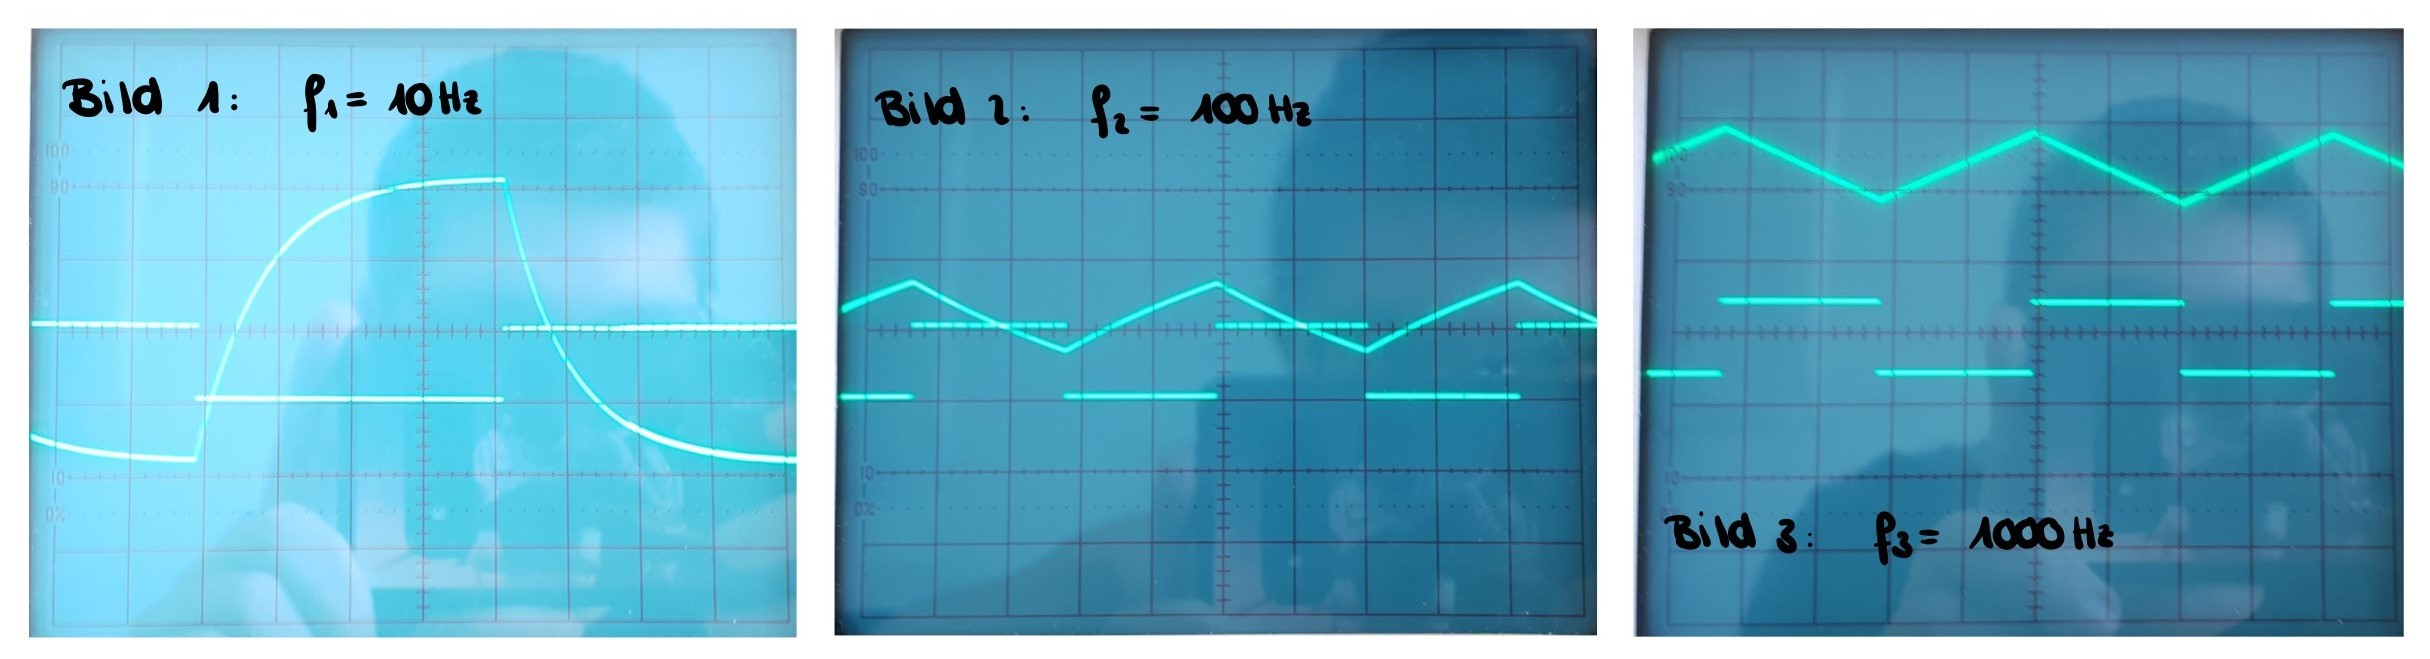
\includegraphics[width=0.9\textwidth]{Auswertung-Anna/Integration.jpg}
        \caption{Aufnahmen des Ozilloskop der Ausgangsspannungen bei angelegter Rechteckspannung für die Frequenzen $f_1 = 10\,\text{Hz}$ (Bild1), $f_2 = 100\,\text{Hz}$ (Bild2) und $f_3 = 1000\,\text{Hz}$ (Bild3).}
        \label{img:Integration}
    \end{center}
    \end{figure} 
    
Wie aus den oberen Aufnahmen ersichtlich, erkennt man
bei dem ersten Bild, $f_1 = 10\,\text{Hz}$, noch keine Integration, man
kann sie höchstens erahnen. Je höher die Frequenzen werden,
umso deutlich zeichnet sich eine Integration ab. Bei Bild 2, 
$f_2 = 100\,\text{Hz}$, erkennt man die Integration der Rechteckspannung gut, jedoch ist
diese deutlicher bei Bild 3,  $f_3 = 1000\,\text{Hz}$. 
Im Allgemeinen kann man sagen, je höher die Frequenz, umso deutlicher ist
die Integration der Rechteckspannung des Eingangssignals.
\newpage
\subsection{Untersuchung des Frequenzgangs}
Als nächstes werden die gemessenen Werte des Frequenzgangs der Verstärkung
mit den theoretisch berechneten verglichen. \\
Hierzu müssen erst die verwendeten Widerstände, 
Kondensatoren und deren Fehler betrachtet werden:\\
\textbf{Fehler des ersten Widerstand} $R_1 = 9,99\,\text{k}\Omega$:
\begin{equation}
    s_{R_1} = \sqrt{s_a^2+s_r^2} = \sqrt{(0,01\,\text{k}\Omega)^2+((9,99\cdot0,01+0,002)\,\text{k}\Omega)^2} = 0,1023\,\text{k}\Omega
\end{equation}
\textbf{Fehler des zweiten Widerstand} $R_2 = 0,999\,\text{M}\Omega$:
\begin{equation}
    s_{R_2} = \sqrt{s_a^2+s_r^2} = \sqrt{(0,001\,\text{M}\Omega)^2+((0,999\cdot0,012+2\cdot10^{-6})\,\text{M}\Omega)^2} = 0,01203\,\text{M}\Omega
\end{equation}
Also ergibt sich:
\begin{align}
    R_1 &= (9,99 \pm 0,10)\,\text{k}\Omega\\
    R_2 &= (1,00 \pm 0,01)\,\text{M}\Omega\\
    C_2 &= 10,17\,\text{nF}
\end{align}
Der Wert des Kondensators wurde nachgemessen, leider lag keine Anleitung vor. 
Zudem wäre der Fehler im nF - Bereich und somit verschwindend gering. \\

Des Weiteren wurde die \textbf{Ausgangsspannung} bestimmt:\\
Die gemessene Ausgangsspannung, die im Protokoll angegeben ist, 
wird im folgenden als '$Y$' bezeichnet.
$\tilde{U}_\text{a}$ bezeichnet die eingestellte Skalierung in '$\frac{V}{div}$'.
\begin{align}
    U_\text{a} &= \tilde{U}_\text{a} \cdot Y \text{div}\\
    s_{\text{U}_\text{a}} &= \sqrt{(0,03\cdot \text{U}_\text{a})^2+(\tilde{U}_\text{a}\cdot 0,5\,\text{div})^2}
\end{align}
Wobei die $3\%$, der systematische Restfehler des Oszilloskops, und die '$0,5\,\text{div}$' den Ablesefehler beschreiben.\\
Der Wert der \textbf{Eingangsspannung} blieb konstant bei $U_\text{e} = 20\,\text{mV}$.\\
Fehler der Eingangsspannung:
\begin{equation}
    s_{\text{U}_\text{e}} = \sqrt{(0,03\cdot 0,02\,V)^2+(0,02\,\frac{\text{V}}{\text{div}} \cdot 0,5\,\text{div})^2} = 1,1661\,\text{mV}
\end{equation} 
\begin{equation}
   \Rightarrow U_\text{e} = (20 \pm 1)\,\text{mV}
\end{equation}
Die \textbf{experimentelle Verstärkung $\upsilon$} wird berechnet, indem man die Ausgangsspannung $U_\text{a}$ durch 
die Eingangsspannung $U_e = 0,02\,V$ teilt. \\
Der Fehler der experimentellen Verstärkung wird wie folgt berechnet:
\begin{equation}
    s_{\upsilon} = \sqrt{(\frac{\partial \upsilon}{\partial U_\text{a}} \cdot s_{\text{U}_\text{a}})^2 +\frac{\partial \upsilon}{\partial U_\text{e}} \cdot s_{\text{U}_\text{e}})^2 } = \sqrt{(\frac{1}{U_\text{e}}\cdot s_{\text{U}_\text{a}})^2 + (\frac{U_\text{a}}{U_\text{a}^2}\cdot s_{\text{U}_\text{e}})^2}
\end{equation}
Zum Schluss wird noch die \textbf{theoretische Verstärkung $\upsilon_{theo}$} berechnet, hierzu wird die Formel 
aus den Fragen zur Vorbereitung verwendet:
\begin{equation}
    \upsilon_{theo} = \frac{R_2}{R_1} \cdot \frac{1}{\sqrt{1 + (C_2 \cdot \omega \cdot R_2)^2}}
\end{equation}
Wobei die Kreisfrequenz $\omega = 2\pi \cdot f$ verwendet wird.\\
Der Fehler von $\upsilon_{theo}$ kann vernachlässigt werden.
\newpage
Die berechneten Werte werden in der Tabelle \ref{tab:Umkehrintegrator} eingetragen.\\
\begin{table}[h]
    \centering
      \begin{tabular}{c||c|c|c|c|c|c|c}
      $f$ in Hz & $U_\text{a}\:\text{in}\:\text{V}$   & $s_{\text{U}_\text{a}}\:\text{in}\:\text{V}$ & $\omega\:\text{in}\:\frac{1}{\text{s}}$& $s_{\omega}\:\text{in}\:\frac{1}{\text{s}}$ & $\upsilon$ & $s_{\upsilon}$ & $\upsilon_\text{theo}$\\
      \hline
      1     & 2,000 & 0,504 & 6,283 & 0,003 & 100,0 & 25,480 & 99,797 \\
      30    & 1,000 & 0,252 & 188,496 & 0,075 & 50,0  & 12,740 & 46,287 \\
      50    & 0,620 & 0,102 & 314,159 & 0,126 & 31,0  & 5,228 & 29,897 \\
      60    & 0,500 & 0,101 & 376,991 & 0,151 & 25,0  & 5,149 & 25,262 \\
      70    & 0,440 & 0,101 & 439,823 & 0,176 & 22,0  & 5,116 & 21,839 \\
      80    & 0,400 & 0,101 & 502,655 & 0,201 & 20,0  & 5,096 & 19,216 \\
      90    & 0,360 & 0,101 & 565,487 & 0,226 & 18,0  & 5,078 & 17,148 \\
      100   & 0,320 & 0,051 & 628,319 & 0,251 & 16,0  & 2,621 & 15,476 \\
      110   & 0,280 & 0,100 & 691,150 & 0,276 & 14,0  & 5,047 & 14,099 \\
      120   & 0,260 & 0,100 & 753,982 & 0,302 & 13,0  & 5,041 & 12,944 \\
      300   & 0,100 & 0,050 & 1884,956 & 0,754 & 5,0   & 2,512 & 5,215 \\
      500   & 0,060 & 0,025 & 3141,593 & 1,257 & 3,0   & 1,259 & 3,131 \\
      700   & 0,050 & 0,025 & 4398,230 & 1,759 & 2,5   & 1,256 & 2,237 \\
      1000  & 0,032 & 0,010 & 6283,185 & 2,513 & 1,6   & 0,506 & 1,566 \\
      1500  & 0,020 & 0,010 & 9424,778 & 3,770 & 1,0   & 0,502 & 1,044 \\
      2000  & 0,016 & 0,010 & 12566,371 & 5,027 & 0,8   & 0,502 & 0,783 \\
      2500  & 0,012 & 0,010 & 15707,963 & 6,283 & 0,6   & 0,501 & 0,627 \\
      3000  & 0,012 & 0,010 & 18849,556 & 7,540 & 0,6   & 0,501 & 0,522 \\
      4000  & 0,008 & 0,010 & 25132,741 & 10,053 & 0,4   & 0,500 & 0,392 \\
      5000  & 0,008 & 0,010 & 31415,927 & 12,566 & 0,4   & 0,500 & 0,313 \\
      6000  & 0,006 & 0,010 & 37699,112 & 15,080 & 0,3   & 0,500 & 0,261 \\
      7000  & 0,006 & 0,010 & 43982,297 & 17,593 & 0,3   & 0,500 & 0,224 \\
      8000  & 0,004 & 0,010 & 50265,482 & 20,106 & 0,2   & 0,500 & 0,196 \\
      9000  & 0,004 & 0,010 & 56548,668 & 22,619 & 0,2   & 0,500 & 0,174 \\
      10000 & 0,004 & 0,010 & 62831,853 & 25,133 & 0,2   & 0,500 & 0,157 \\
      \end{tabular}
      \caption{Werte des Frequenzgangs der Verstärkung des Umkehrintegrators.}
      \label{tab:Umkehrintegrator}
  \end{table}\newpage
Im nächsten Schritt wird die experimentelle Verstärkung gegen die berechnete Kreisfrequenz $\omega$ 
doppeltlogarithmisch aufgetragen, zusätzlich wird die theoretisch berechnete Verstärkung mit in 
die Grafik (\ref{fig: UmkehrintegratorDiagramm}) eingezeichnet.
  \begin{figure}[h]
    \centering\scalebox{1}{% GNUPLOT: LaTeX picture with Postscript
\begingroup
  % Encoding inside the plot.  In the header of your document, this encoding
  % should to defined, e.g., by using
  % \usepackage[cp1252,<other encodings>]{inputenc}
  \inputencoding{cp1252}%
  \makeatletter
  \providecommand\color[2][]{%
    \GenericError{(gnuplot) \space\space\space\@spaces}{%
      Package color not loaded in conjunction with
      terminal option `colourtext'%
    }{See the gnuplot documentation for explanation.%
    }{Either use 'blacktext' in gnuplot or load the package
      color.sty in LaTeX.}%
    \renewcommand\color[2][]{}%
  }%
  \providecommand\includegraphics[2][]{%
    \GenericError{(gnuplot) \space\space\space\@spaces}{%
      Package graphicx or graphics not loaded%
    }{See the gnuplot documentation for explanation.%
    }{The gnuplot epslatex terminal needs graphicx.sty or graphics.sty.}%
    \renewcommand\includegraphics[2][]{}%
  }%
  \providecommand\rotatebox[2]{#2}%
  \@ifundefined{ifGPcolor}{%
    \newif\ifGPcolor
    \GPcolorfalse
  }{}%
  \@ifundefined{ifGPblacktext}{%
    \newif\ifGPblacktext
    \GPblacktexttrue
  }{}%
  % define a \g@addto@macro without @ in the name:
  \let\gplgaddtomacro\g@addto@macro
  % define empty templates for all commands taking text:
  \gdef\gplbacktext{}%
  \gdef\gplfronttext{}%
  \makeatother
  \ifGPblacktext
    % no textcolor at all
    \def\colorrgb#1{}%
    \def\colorgray#1{}%
  \else
    % gray or color?
    \ifGPcolor
      \def\colorrgb#1{\color[rgb]{#1}}%
      \def\colorgray#1{\color[gray]{#1}}%
      \expandafter\def\csname LTw\endcsname{\color{white}}%
      \expandafter\def\csname LTb\endcsname{\color{black}}%
      \expandafter\def\csname LTa\endcsname{\color{black}}%
      \expandafter\def\csname LT0\endcsname{\color[rgb]{1,0,0}}%
      \expandafter\def\csname LT1\endcsname{\color[rgb]{0,1,0}}%
      \expandafter\def\csname LT2\endcsname{\color[rgb]{0,0,1}}%
      \expandafter\def\csname LT3\endcsname{\color[rgb]{1,0,1}}%
      \expandafter\def\csname LT4\endcsname{\color[rgb]{0,1,1}}%
      \expandafter\def\csname LT5\endcsname{\color[rgb]{1,1,0}}%
      \expandafter\def\csname LT6\endcsname{\color[rgb]{0,0,0}}%
      \expandafter\def\csname LT7\endcsname{\color[rgb]{1,0.3,0}}%
      \expandafter\def\csname LT8\endcsname{\color[rgb]{0.5,0.5,0.5}}%
    \else
      % gray
      \def\colorrgb#1{\color{black}}%
      \def\colorgray#1{\color[gray]{#1}}%
      \expandafter\def\csname LTw\endcsname{\color{white}}%
      \expandafter\def\csname LTb\endcsname{\color{black}}%
      \expandafter\def\csname LTa\endcsname{\color{black}}%
      \expandafter\def\csname LT0\endcsname{\color{black}}%
      \expandafter\def\csname LT1\endcsname{\color{black}}%
      \expandafter\def\csname LT2\endcsname{\color{black}}%
      \expandafter\def\csname LT3\endcsname{\color{black}}%
      \expandafter\def\csname LT4\endcsname{\color{black}}%
      \expandafter\def\csname LT5\endcsname{\color{black}}%
      \expandafter\def\csname LT6\endcsname{\color{black}}%
      \expandafter\def\csname LT7\endcsname{\color{black}}%
      \expandafter\def\csname LT8\endcsname{\color{black}}%
    \fi
  \fi
    \setlength{\unitlength}{0.0500bp}%
    \ifx\gptboxheight\undefined%
      \newlength{\gptboxheight}%
      \newlength{\gptboxwidth}%
      \newsavebox{\gptboxtext}%
    \fi%
    \setlength{\fboxrule}{0.5pt}%
    \setlength{\fboxsep}{1pt}%
\begin{picture}(7200.00,5040.00)%
    \gplgaddtomacro\gplbacktext{%
      \csname LTb\endcsname%%
      \put(946,704){\makebox(0,0)[r]{\strut{}$0.01$}}%
      \put(946,1439){\makebox(0,0)[r]{\strut{}$0.1$}}%
      \put(946,2173){\makebox(0,0)[r]{\strut{}$1$}}%
      \put(946,2908){\makebox(0,0)[r]{\strut{}$10$}}%
      \put(946,3642){\makebox(0,0)[r]{\strut{}$100$}}%
      \put(946,4377){\makebox(0,0)[r]{\strut{}$1000$}}%
      \put(1078,484){\makebox(0,0){\strut{}$1$}}%
      \put(2103,484){\makebox(0,0){\strut{}$10$}}%
      \put(3128,484){\makebox(0,0){\strut{}$100$}}%
      \put(4154,484){\makebox(0,0){\strut{}$1000$}}%
      \put(5179,484){\makebox(0,0){\strut{}$10000$}}%
      \put(6204,484){\makebox(0,0){\strut{}$100000$}}%
    }%
    \gplgaddtomacro\gplfronttext{%
      \csname LTb\endcsname%%
      \put(209,2761){\rotatebox{-270}{\makebox(0,0){\strut{}$\nu$}}}%
      \csname LTb\endcsname%%
      \put(6748,2761){\rotatebox{-270}{\makebox(0,0){\strut{}}}}%
      \csname LTb\endcsname%%
      \put(3885,154){\makebox(0,0){\strut{}$\omega\,\left(\frac{1}{\text{s}}\right)$}}%
      \csname LTb\endcsname%%
      \put(3885,4819){\makebox(0,0){\strut{}}}%
      \csname LTb\endcsname%%
      \put(132,-110){\makebox(0,0)[l]{\strut{}}}%
      \csname LTb\endcsname%%
      \put(5706,4646){\makebox(0,0)[r]{\strut{}Messwerte}}%
      \csname LTb\endcsname%%
      \put(5706,4426){\makebox(0,0)[r]{\strut{}Erwartete Werte}}%
      \csname LTb\endcsname%%
      \put(3885,42893){\makebox(0,0){\strut{}}}%
    }%
    \gplbacktext
    \put(0,0){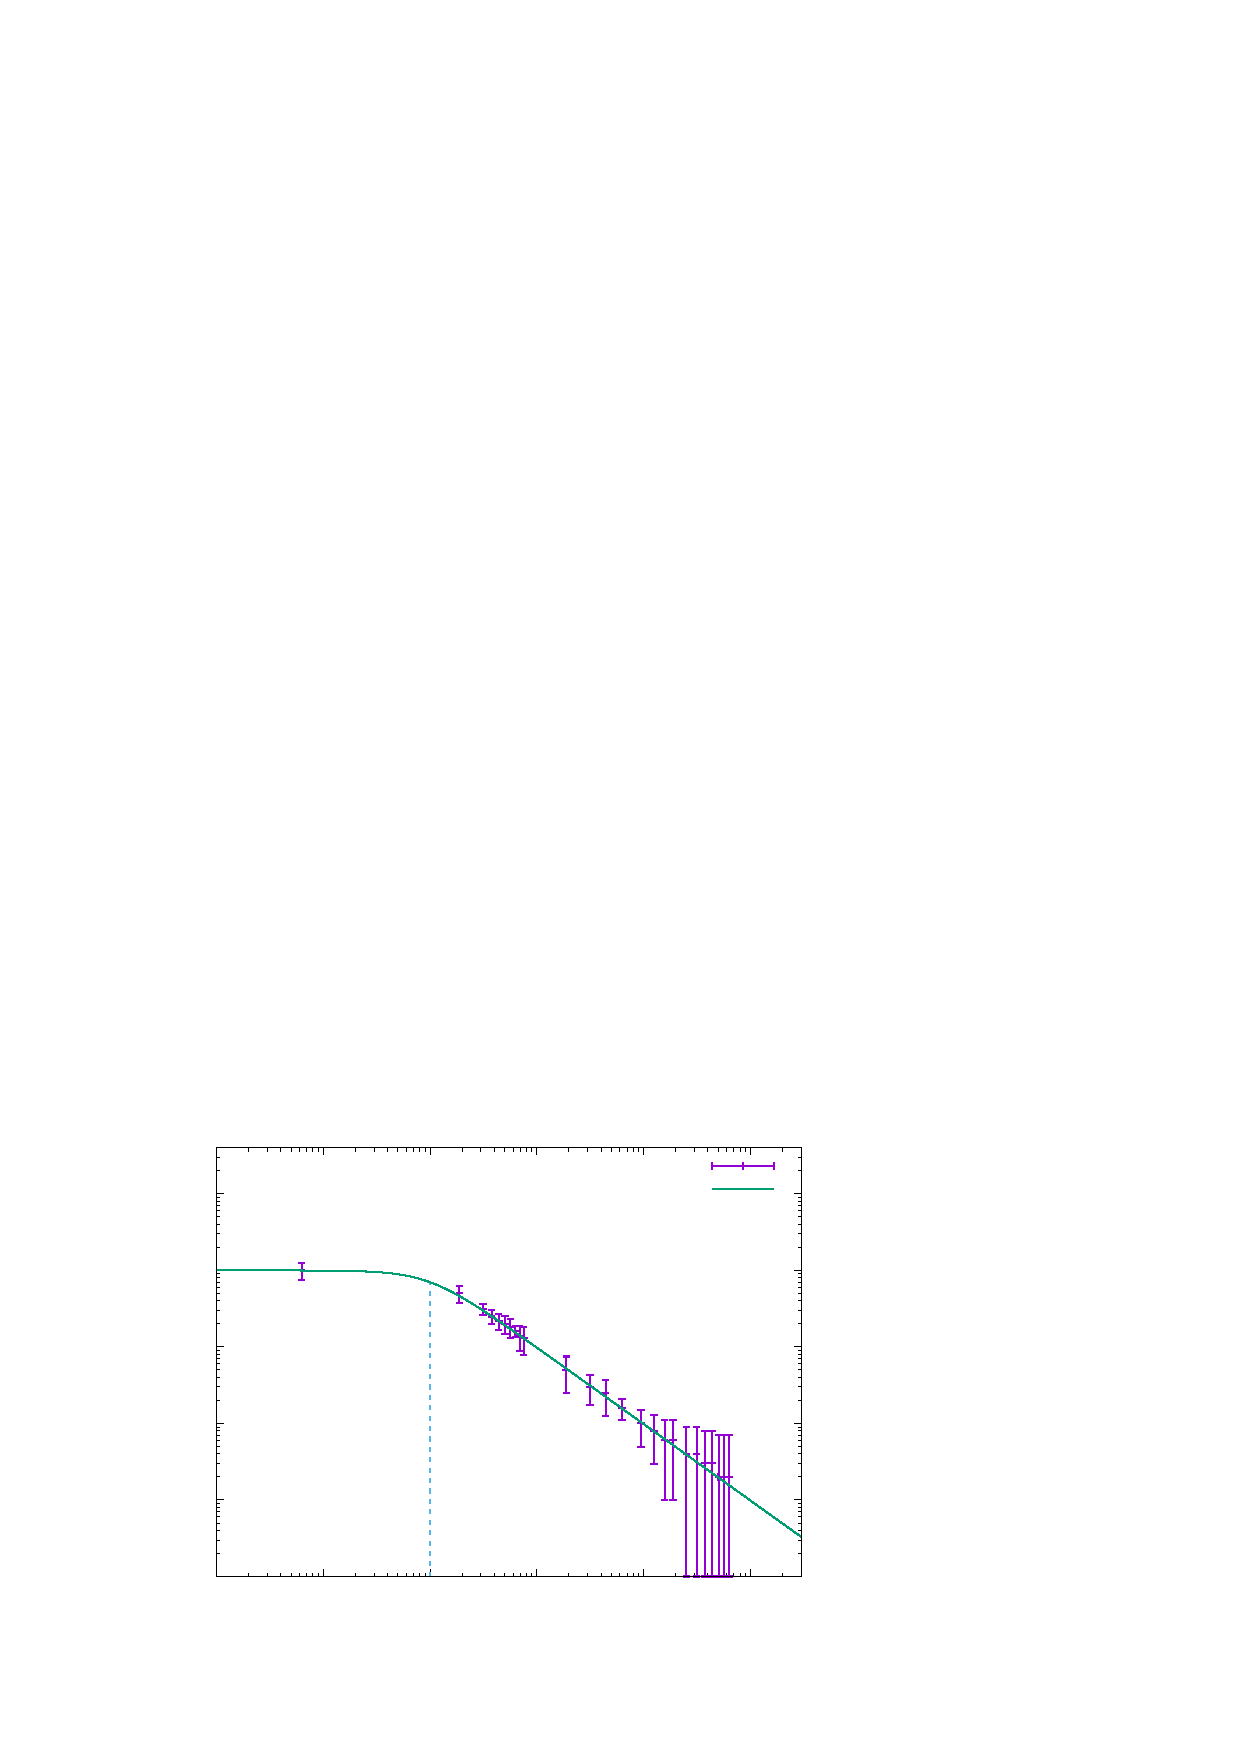
\includegraphics[width={360.00bp},height={252.00bp}]{Integrierer_final}}%
    \gplfronttext
  \end{picture}%
\endgroup
}
    \caption{Die Verstärkung des Umkehrintegrators gegen die Kreisfrequenz doppeltlogarithmisch aufgetragen. }
    \label{fig: UmkehrintegratorDiagramm}
\end{figure}

Wie man erkennen kann, passen die theoretisch berechneten Werte und die experimentell
gemessenen Werte überein, vor allem, wenn man die Fehler mit berücksichtigt.
Die theoretische Grenzfrequenz liegt bei etwa $\omega_\text{theo} = \frac{1}{C_2 \cdot R_2} \approx 99,32\,\frac{1}{\text{s}}$, diese stimmt, 
mit der experimentell bestimmten Wert von $\omega_\text{grenz} \approx 100 \frac{1}{\text{s}}$ überein, vgl. Grafik. Hierbei ist allerdings zu erwähnen, 
dass in dem entsprechenden Frequenzbereich kaum Messwerte vorliegen
und somit die genaue Bestimmung schwierig ist. \\
Wenn man nun von diesem geschätzen Wert ausgeht heißt dies, dass unsere Schaltung ab ungefähr $\omega \approx 100\,\frac{1}{\text{s}}$ als Integrator fungiert, also ungefähr ab einer Frequenz von $f_\text{grenz} \approx 16\,\text{Hz}$ .
Dies stimmt auch mit den in 3.2.1 Qualitativen Beobachtungen überein.